\section{Understanding Instability in Looped Architectures}
\label{sec:dynamical-systems}

\begin{figure*}[t]
    \centering
    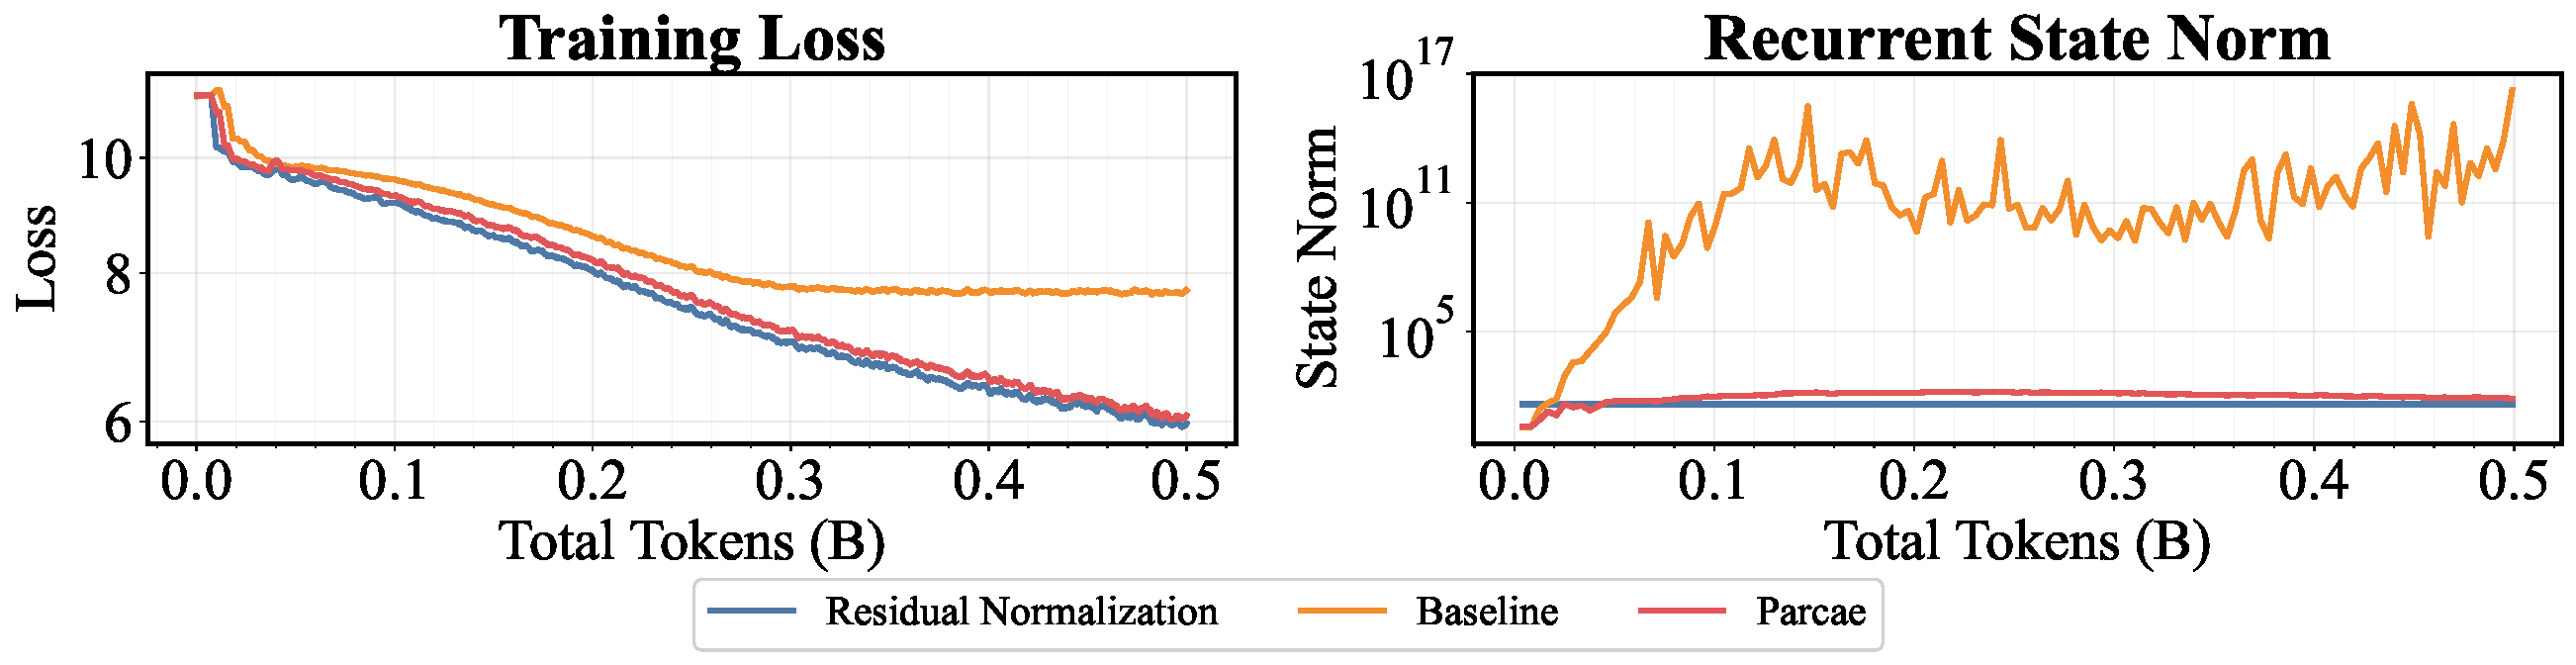
\includegraphics[width=\linewidth]{figures/main/instability_comparison.pdf}
    \caption{\textbf{Training Instability of Looped Architectures.} (\emph{left}) Pre-Norm looped models diverge, while residual norm. and \sysname converge. (\emph{right}) Instability stems from an exploding recurrent state norm $||h_T||_2$, the hidden embedding norm after $T$ recurrences.}
    \label{fig:instability}
    \vspace{-0.8em}
\end{figure*}




In this section, we study the instability of looped architectures. Using an LTI view over the residual, we find that instability stems from an unconstrained residual state explosion (\cref{fig:instability}; \cref{tab:hyperparameters}~[\emph{Baseline}]; \cref{sec:stability-ablations}).
While residual normalization helps mitigate this issue, it requires sensitive hyperparameter tuning (\cref{tab:hyperparameters} [\emph{Res. Norm}]), similar to fixed-depth transformers \citep{xu2019understandingimprovinglayernormalization, xiongLayerNormalizationTransformer2020}.
Using this LTI framework, we derive stability conditions for the eigenvalues of $\dA$. We find that prior work does not satisfy these conditions for $\dA$, which we empirically verify creates major state explosion (\cref{fig:spectral-norm}).

\paragraph{Dynamical System over Residual Stream.} Our key insight is to recast the forward pass as a dynamical system over the residual stream. Consider a transformer-based looped model as defined in \cref{sec:rdm-basics} for language modeling, where \prelude is an embedding layer that maps a sequence of tokens $s \in V^n$ into embedding space $e \in \R^{n \times d_h}$, \coda is a projection head that maps into probability space $g: d_h \to |V|$, and \recurrent is parameterized with $L$ transformer blocks. While several methods of input injection could condition \recurrent on $e$, building on prior work \citep{yang2024loopedtransformersbetterlearning, geiping_scaling_2025, mcleish_retrofitted_recurrence}, we focus on linear methods of injection (e.g., $\mathcal{R}(h_t, e) = \mathcal{R}(W_1 h_t + W_2 e)$, where $W_1 \in \R^{d_h  \times d_h}$ and $W_2 \in \R^{d_h \times d_e}$).\footnote{Both addition \citep{yang2024loopedtransformersbetterlearning} and concatenation \citep{geiping_scaling_2025} fall under this framework.}


Recall that \recurrent denotes the full recurrent update $h_{t+1} = \mathcal{R}(h_t,e)$, encompassing all transformer operations, including residual connections. 
The recurrent update can be exactly formulated as a non-linear time-variant dynamical system of the form $h_{t} = \dA h_{t-1} + \dB e + \overline{\mathcal{R}}(h_{t-1}, e), ~ y_t = \C h_t,$
where $\C \in R^{d_c \times d_h}$ decouples the \coda and \recurrent embedding dimension (i.e.~$p=\mathcal{C}(\C(h_T))$). 
This derivation is shown in \cref{sec:derivation-instabilty}. Though this formulation does not immediately elucidate instability,
linearizing of this system (i.e., dropping $\overline{\mathcal{R}}$) yields a discrete LTI system of the form:
\begin{equation}
h_{t+1} = \dA h_t + \dB e
\label{eq:lti}
\end{equation}

\begin{table}[!t]
    \centering
    \renewcommand{\arraystretch}{1.15}
    \small
    \begin{tabular*}{\textwidth}{@{\extracolsep{\fill}} l  c  c c c @{}}
    \toprule
         Method & $\dA$ & $\dB$ & $\rho(\dA)$ & LTI Stability \\
    \midrule
         Addition & $I$ & $I$ & $\rho(\dA) = 1$ &  \emph{marginally-stable} \\
         Concatenation & $\R^{d_h \times d_h}$ & $\R^{d_h \times d_e}$& $\rho(\dA) \in \R$  & \emph{unstable} \\
         \sysname (ours) & $\text{ZOH}(\texttt{Diag}(-\exp(\R^{d_h}))$ & $\text{Euler}(\R^{d_h \times d_e})$ &$\rho(\dA) < 1 $ & \emph{stable} \\
    \bottomrule
    \end{tabular*}
    \caption{\textbf{Comparison of Prior Update Rule Stability based on LTI Representation.}}
    \label{tab:stability-equation-comparison}
\end{table}

\begin{table}[!t]
    \centering
    \begin{minipage}[t]{0.4\textwidth}
        \vspace{0pt}
        \centering
        \small
        \begin{tabular}{lccc}
            \toprule
            \textbf{LR} & \textbf{Base} & \textbf{Res. Norm} & \textbf{Parcae} \\
            \midrule
            2e-4 & \cmark & \cmark & \cmark \\
            4e-4 & \xmark & \cmark & \cmark \\
            6e-4 & \xmark & \xmark & \cmark \\
            8e-4 & \xmark & \xmark & \cmark \\
            1e-3 & \xmark & \xmark & \cmark \\
            \bottomrule
        \end{tabular}
        \caption{\textbf{Hyperparameter Instability.} Convergence across learning rates for baseline RDMs, Res. Norm RDMs, and \sysname. \sysname is more robust to hyperparameter selection. Full logs are in \cref{sec:stability-ablations}.}
        \label{tab:hyperparameters}
    \end{minipage}
    \hfill
    \begin{minipage}[t]{0.56\textwidth}
        \vspace{-6pt}
        \centering
        \makeatletter\def\@captype{figure}\makeatother
        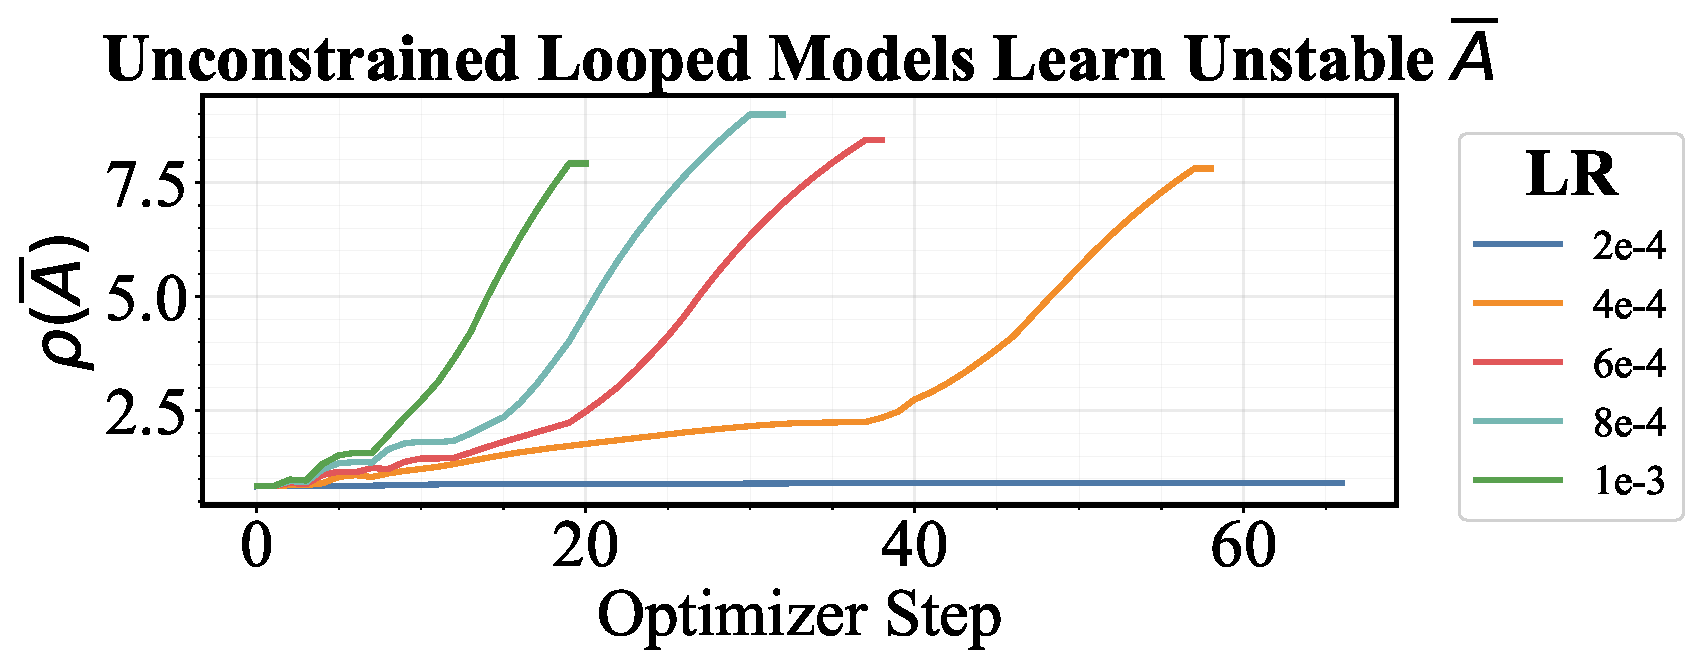
\includegraphics[width=\linewidth]{figures/main/spectral_radius_lr_sweep.pdf}
        \vspace{-1.6em}
        \caption{\textbf{Spectral Radius of Unconstrained $\protect\dA$.} For a Pre-Norm RDM, we plot the $\rho(\dA)$ throughout training using different learning rates, observing divergent runs learn $\rho(\dA) > 1$. The state explosion, in \cref{fig:instability} is thus directly linked to $\dA$.}
        \label{fig:spectral-norm}
    \end{minipage}
    \vspace{-0.7em}
\end{table}

\paragraph{State Explosion from Unconstrained $\dA$ and $\dB$.}
Analyzing the stability of \cref{eq:lti} identifies $\rho(\dA)$ as a critical factor governing instability.
As shown in \cref{tab:stability-equation-comparison}, prior work \citep{geiping_scaling_2025, yang2024loopedtransformersbetterlearning} chooses parameterizations of $\dA$ such that $\rho(\dA)=1$ or $\rho(\dA)$ is unconstrained. Critically, these are \emph{marginally-stable} or \emph{unstable parameterizations}.

\cref{fig:spectral-norm} and \cref{tab:hyperparameters} confirm this empirically:
divergent runs learn a spectral radius of $\rho(\dA) \geq 1$, with convergent runs maintaining $\rho(\dA) < 1$, affirming that LTI stability constraints are necessary. 
Finally, at scale, we observe loss spikes late in training 
(e.g., after 170k steps), which we address by normalizing the input to $\dB$ (see \cref{sec:prelude-norm} for ablation).





